\documentclass[a4paper,pt12]{article}
\usepackage{graphicx}
\usepackage{url}
\usepackage{placeins}

\begin{document}
\author{Pascal Stammer, Mats Richter, Benjamin Henne}
\title{Final Project: A Comparison Of Siamese Oneshot Classification With Softmax Classification using Deep Neural Networks}

\maketitle

\begin{abstract}
Learning from datasets with sparse samples for individual classes and high imbalance in the distribution of classes is a prominent issue in deep learning and machine learning in general. Modern deep learning architectures routinely require thousands of data points per class to learn generalizing concepts. Siamese Networks are an attempt to create a classifier that is very robust towards class imbalances and (in theory) able to distinguish classes by only seeing a single sample of one of the two classes, coined "One-shot classification". This work evaluates the classification performance of a siamese neural network by comparing the performance measures to a very similar softmax-classification convolutional neural network. We will compare the baseline performance differences between the networks on a balanced dataset and further compare the performance on highly imbalanced data.

\end{abstract}

\section{Task description}
In most machine learning approaches large amounts of data are key to achieve acceptable or even human-level performance in classification tasks.
However, in contrast to the plethora of large pre-built data sets that exist for well-defined toy problems, the amount of data available for many real world applications is scarce at best. Other common hurdles are a general lack of class balance within the data and the expensive retraining of the entire model in case more classes are added after the training is complete.
To address the issues of small training sets, unbalanced data and the possible need for retraining, Fei-Fei et al. (2003) developed a technique called One-shot Classification, in which the network is only allowed to observe a single sample of each class in the data set before making its prediction. It is important to distinguish this from the concept of Zero-shot Classification, in which the model has no access at all to target class samples (Palatucci et al., 2009).
In this project we replicate the deep neural network proposed in Koch et. al, 2015 called Siamese Neural Network. To validate its one-shot classifications potential and its ability to solve problems containing unbalanced data sets we compare the classification performance of a simple convolutional neural network and a siamese neural network with the same convolutional network structure.
In order to properly examine the performance, we chose to use the EMNIST (Extended MNIST) data set as proposed by Cohen et al. in 2017. It consists of around 700,000 images of handwritten digits and letters of 62 classes and is fairly unbalanced. This provides a more solid base to evaluate classification performance on an unbalanced data set rather than using MNIST, and to compare this performance to classical approaches used in the deep learning community. We decided against using the original Omniglot data set for simplicity's sake.


\section{Related work and similar approaches}
According to Koch et al. (2015), research into one-shot classification is still in its infancy and not of particular import to the deep learning community.

The cornerstone paper of one-shot learning dates back to the early 2000's by Li Fei-Fei et al. They developed a Bayesian framework for one-shot classification that used previously learned classes to help forecast future ones, which displayed strong generalization properties when applied to classes with acutely low sample sizes. (Fei-Fei et al., 2003; Fei-Fei et al., 2006).

In a few more contemporary papers, Lake et al. came up with a method called Hierarchical Bayesian Program Learning (2011; 2012; 2013), a technique for one-shot character recognition that achieves human-level performance by representing learned concepts that best explain observed examples under a Bayesian criterion. Another approach they designed uses a generative Hierarchical Hidden Markov model in combination with a Bayesian inference procedure to recognize spoken words from unknown speakers (2014).

Other than image classification, the application of one-shot learning has also been considered in other transfer learning approaches. Maas and Kemp used Bayesian networks to predict passenger attributes for historic Ellis Island travel data (2009), Wu and Dennis applied it to path-planning algorithms of robotic actuation (2012) and Lim tried to model human-level concept extraction for data sets with very small class sample sizes by creating an adaptive measure of how much each learned category should be weighted by each training sample in the loss function (2012).

Very few alternatives to the Bayesian One-shot Learning approach exist currently. A notably different approach presented by Miller et al at ICCV 2000 incorporates knowledge transfer via model parameters to learn new object categories which are visually similar to previously learned categories.

\section{Theoretical basis and used procedures}
The task of one-shot classification is to learn to distinguish between the class-identity of image pairs, which is called standard verification task for image recognition (Koch et. al., 2015). This means that the model judges pairs of images based on whether they belong to the same or a different class according to the probabilistic output of the model. Additionally, if samples of new classes arise after training completion, the same model can be used to classify those new samples (Koch et. al., 2015). In the original paper the authors new samples would be paired with known samples, one per class. Then the pairing with the highest score is selected as the pair with the highest probability and the class of the known sample is used as class for the new sample. We altered this approach such that we present more than one known sample of one class and average over those groupings of pairs such that we can select the pairing with the highest average probability.

First introduction of siamese neural networks dates back to the early 1990s by Bromley and LeCun, used to tackle the task of signature verification. A twin neural network with shared parameters and architecture is the main building block of a siamese neural network. It accepts two distinct inputs and the output is joined by an energy function. The approximate function computes the distance between the two high level feature representation of the inputs. Each part of the twin neural network projects the input onto a projection feature space. To prevent that two equal inputs of two different parts of the twin network would be projected into two different regions of the feature vector space, the weights are shared between the two parts of the network. Furthermore, the network is symmetric such that the computed metric will be the same, irrespective which input network was used for the pair of inputs.

For the energy function multiple approaches exists. LeCun et al. used a contrastive energy function which decreases the energy of sample pairs of the same class and increase the energy of those of different classes. Koch et al. used the L1-distance between the two twin network respective outputs $h1$ and $h2$ combined with a sigmoid activation which leads to using the sigmoidal cross entropy.

Equal to Koch et al., our models use multiple convolutional layers before the fully-connected layers and the energy function. Convolutional layers are a good fit because they achieve very good performance in image recognition task. Furthermore, they are able to reduce the number of free parameters because of the local connectivity properties of convolutional layers and learn a high level feature representation of the image which could rule out the problems of the "Curse of dimensionality" because the number of input features in the fully-connected layers will be reduced. In addition, the model may be not that sensible to outliers and transformations of the input image because it groups the single pixel values to the high level features mentioned above (Koch et al., 2015).

\subsection{Siamese Neural Networks}

\section{Experiments}
The experiments are aimed to look into the differences in learning behaviour between deep neural networks and siamese deep neural networks. We therefore used two simple and very similar showcase architectures to make this comparison as clear as possible. We used the MNIST and the quantitatively larger EMNIST datasets as our data basis for our experiments. We altered the datasets class balance and the number of classes to compare the performance of both networks in increasingly difficult situations with regards to the structure of the dataset while keeping the data itself relatively simple.  

\subsection{Network Architectures}
In order to make the performance of both networks comparable and keep the complexity of the models as simple as possible, both architectures are exact clones apart from the siamese properties. We also refused to use more complex architectural features like highway connections or multiple paths like in the Inception architectures, to rule out more complex influences on the typical learning behaviour of convolutional neural networks.

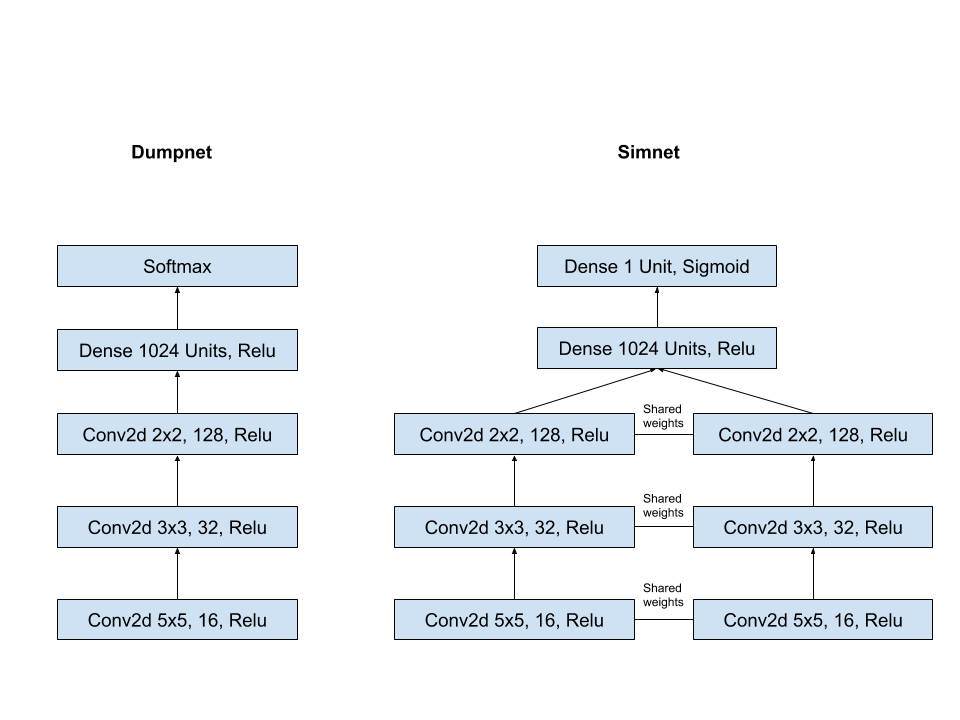
\includegraphics[scale=0.3]{nets.png}

\subsubsection{Dumbnet}
This network is our baseline model for comparing and evaluating the performance of the siamese network.  It consists of 3 convolutional layer with ReLU activation functions, valid padding, and increasing filter size. \newline
The output of the convolutional part (from now on called stem) of the network is read out by a single dense layer with 1024 units and ReLU activation function and fed into a 10 way (MNIST) or 62 way (EMNIST) softmax. For optimization, an Adam Optimizer with default parameters was used.

\subsubsection{Simnet}
Simnet is derived from the Dumbnet architecture. The siamese part consists of two stems, each identical to the one of Dumbnet. Each stem receives a single image as input. The readout is concatenated and put into a dense layer of 1024 units with ReLU activation function and a single unit output with sigmoidal activation function. \newline
Simnet is trained by randomly arranging the images into pairs. The labels are created like in \cite{siamese}, non-matching original labels result in 1, matching original labels result in 0. This process is repeated for each epoch of training. \newline
The loss of the network is weighted by $1:10$ (MNIST) or $1:62$ (EMNIST) in favour of matching original labels, due to the statistical probability of two random images belonging to the same class. This implies the assumption of balanced classes, even though the EMNIST dataset is not balanced. This is intentional, since no sample or class weights are applied on the loss of Dumbnet, which implies also the assumption of balanced classes. \newline
A normal Gradient Decent optimizer was used, since Adam lead to instabilities in the learning dynamics. The default values were kept the same.


\subsection{Data and Experimental Setups}

\subsubsection{MNIST Experiments}

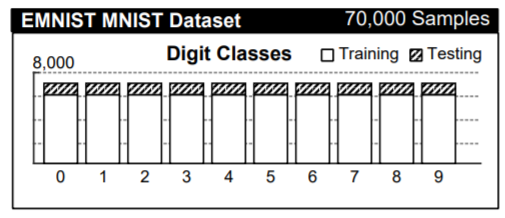
\includegraphics[scale=0.8]{mnist.png}

The MNIST dataset is one of the standard datasets in machine learning and deep learning. It is a balanced dataset consisting of binary, square images with a size of 28x28 pixels. There are ten classes resembling handwritten digits from zero to nine. The dataset is balanced and known to be very solvable for simple computer vision algorithms with little noise and no misclassifications in the ground truth. \newline
The MNIST performance serves as baseline of performance on a solvable, balanced classification problem. \newline
The experiments were conducted with the default parameters and 10 Epochs of training on both algorithms. Simnet received on test time 10 samples per class and averaged over the samples to generate the final classification. The batch size for both networks was fixed to 256 data points per mini batch.

\subsubsection{EMNIST Experiments}

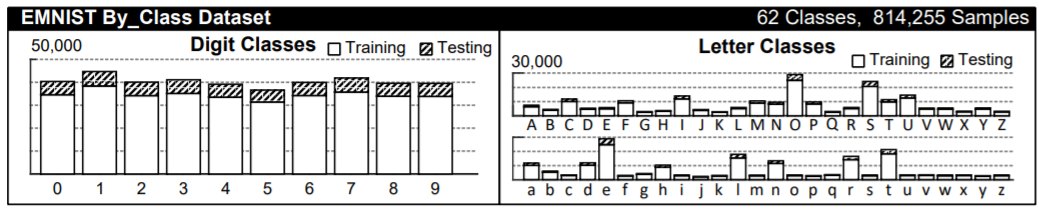
\includegraphics[scale=0.6]{emnist.png}

EMNIST is a novel extension for the MNIST dataset. We used the by-class version of the dataset with 62 classes, containing additional classes for handwritten letters (lower and capital are treated as separate classes). The most important property of this dataset is the relatively close resemblance to MNIST by simultaneously being a more complex classification problem with strong imbalances between the classes. \newline
The experimental setup is identical to MNIST with the exception of the number of epochs for Simnet, which was increased to 100, since Simnet took longer to converge.


\section{Results}
In this chapter, we will present the results of the experiments. First we will discuss the MNIST results and deduct the performance differences on balanced datasets. We will then move on to the EMNIST experiments and compare the results to MNIST-experiments and how strong imbalances impact the learning behaviour of both algorithms.

\subsubsection{MNIST Experiments}
\begin{center}
    \begin{tabular}{| l | l | l | }
    \hline
    Network & Accuracy & Weighted Accuracy \\ \hline
    Dumbnet & 96.98\% & not needed (balanced) \\ \hline
	Simnet & 95.78\% & not needed (balanced) \\ \hline
    \end{tabular}
\end{center}

On MNIST both Networks showed very similar performance, but with a slight edge in favour of Dumbnet. The reason for this is likely the probabilistic inference of Simnet. Also Simnet needed a lot more training epochs to converge to a comparable solution. However, this was expected since the dataspace of two digit pairs is a lot larger than the dataspace of single MNIST-Digits. 

\subsubsection{EMNIST Experiments}
\begin{center}
    \begin{tabular}{| l | l | l | }
    \hline
    Network & Accuracy & Weighted Accuracy \\ \hline
    Dumbnet & 82.51\% & 68.
    06\% \\ \hline
	Simnet & 69.42\% & 41.78\% \\ \hline
    \end{tabular}
\end{center}

Suprisingly, the performance on EMNIST decreased drastically for Simnet, meanwhile Dumbnet’s performance also decreased severely, but not nearly as much as Simnet’s. \newline
Finding reasons for this decrease is highly speculative and would require more heterogeneous testing, which are out of scope for this project, to properly verify. The performance on training  time for Simnet is still good with 96\% accuracy on training samples The likeliest cause for the performance decrease is the increase in classes compared to MNIST. Discriminative features learned by Simnet that optimize the recognition of differences between two labels do not generalize on all labels, creating a distance measure that does not distinguish very well between all labels in a way, that would allow good multi-class classification. \newline

\section{Conclusion and Outlook}
In our final project, we implemented a siamese and a convolutional neural network with very similar architectures to compare the performance of both on multi-class classification problems on balanced (MNIST) and imbalanced (EMNIST) datasets. \newline
We showed that the siamese network has very similar multi-class accuracy on MNIST, but this does not translate over to EMNIST, where the siamese network generally failed to give good multi class classification result even though it had a high binary classification accuracy. \newline
For future works it would be interesting to verify these results on different datasets and a more general set of architectures, which was not possible in this work due to time and resource constraints. A deeper look into the interaction of imbalance of data and classification performance would be also interesting to look at, in order to further verify or reject the hypothesised advantage of one-shot classification when dealing with extreme imbalances or single samples in a dataset.

\end{document}